\documentclass{beamer}
\usetheme{Madrid}
\usecolortheme{dolphin}
\usepackage{graphicx}
\usepackage{booktabs}
\usepackage{amsmath}
\usepackage{tikz}

\title{Security Alerting and Monitoring}
\subtitle{Concepts, Tools, and Best Practices}
\author{Instructor Name}
\institute{University/Institution Name}
\date{\today}

\begin{document}

\begin{frame}
\titlepage
\end{frame}

\begin{frame}
\frametitle{Security Alerting \& Monitoring: Protecting Digital Assets in Real-Time}
\begin{itemize}
\item \textbf{Security monitoring} is the continuous observation of systems, applications, and networks to detect security events.
\item Effective monitoring enables organizations to identify and respond to threats before significant damage occurs.
\item Modern security requires 24/7 vigilance across increasingly complex digital environments.
\item The goal is to maintain visibility into all security-relevant activities across the enterprise.
\end{itemize}

\begin{alertblock}{Key Concept}
Security monitoring is not a one-time setup but a continuous process that requires regular assessment and refinement.
\end{alertblock}
\end{frame}

\begin{frame}
\frametitle{Lesson Overview: What We'll Cover}
\begin{itemize}
\item We will explore the fundamental components of security monitoring infrastructure.
\item You will learn how to implement effective security alerting mechanisms that balance sensitivity with precision.
\item This leson covers both technical tools and organizational processes needed for security operations.
\item By the end, you'll understand how to build and maintain a comprehensive security monitoring program.
\end{itemize}

\begin{columns}[T]
\begin{column}{0.5\textwidth}
\textbf{Technical Focus}
\begin{itemize}
\item Monitoring tools
\item Log analysis
\item Alert configuration
\item Vulnerability scanning
\end{itemize}
\end{column}
\begin{column}{0.5\textwidth}
\textbf{Process Focus}
\begin{itemize}
\item Response workflows
\item Remediation procedures
\item Documentation
\item Continuous improvement
\end{itemize}
\end{column}
\end{columns}
\end{frame}

\begin{frame}
\frametitle{Introduction to Security Monitoring: Why It Matters}
\begin{itemize}
\item Security breaches cost organizations an average of \$4.45 million per incident (2023 data).
\item Most successful attacks go undetected for over 200 days without proper monitoring.
\item Regulatory requirements (GDPR, HIPAA, PCI-DSS) mandate security monitoring and incident reporting.
\item Early detection through monitoring significantly reduces the impact and cost of security incidents.
\end{itemize}

\begin{exampleblock}{Real-World Example}
A major retailer detected unusual database query patterns through their monitoring system, identifying an active breach targeting customer payment data before any information was exfiltrated.
\end{exampleblock}
\end{frame}

\begin{frame}
\frametitle{The Security Monitoring Lifecycle}
\begin{itemize}
\item The \textbf{security monitoring lifecycle} is a continuous process of collection, analysis, alerting, and improvement.
\item Data collection forms the foundation, gathering information from diverse sources across the enterprise.
\item Analysis transforms raw data into actionable security intelligence through correlation and context.
\item Response and remediation close the loop by addressing identified threats and vulnerabilities.
\end{itemize}

\begin{center}
\textbf{The Security Monitoring Lifecycle}

\begin{tabular}{ccccc}
Collect & $\rightarrow$ & Analyze & $\rightarrow$ & Alert \\
$\uparrow$ & & & & $\downarrow$ \\
Improve & $\leftarrow$ & Adjust & $\leftarrow$ & Respond \\
\end{tabular}
\end{center}
\end{frame}

\begin{frame}
\frametitle{Monitoring Computing Resources: The Big Picture}
\begin{itemize}
\item \textbf{Computing resources} include all digital assets an organization relies on to conduct business.
\item Comprehensive monitoring requires visibility into systems, applications, and infrastructure components.
\item The scale of modern environments necessitates automated monitoring solutions with intelligent filtering.
\item Different resources require different monitoring approaches based on their criticality and vulnerability profile.
\end{itemize}

\begin{block}{Monitoring Layers}
\begin{tabular}{ll}
\textbf{Layer} & \textbf{Examples} \\
\hline
Systems & Operating systems, endpoints, servers \\
Applications & Web apps, databases, custom software \\
Infrastructure & Networks, cloud services, IoT devices \\
\end{tabular}
\end{block}
\end{frame}

\begin{frame}
\frametitle{Systems Monitoring: Critical Components}
\begin{itemize}
\item \textbf{Systems monitoring} focuses on operating systems, host-based activities, and endpoint behaviors.
\item Key indicators include user authentication events, privilege escalation, and unauthorized software execution.
\item Host-based intrusion detection systems (HIDS) monitor for changes to critical system files and configurations.
\item Endpoint detection and response (EDR) solutions provide detailed visibility into endpoint activities.
\end{itemize}

\begin{alertblock}{Critical System Events to Monitor}
Always prioritize monitoring for account creation, privilege changes, security policy modifications, and unusual process execution patterns.
\end{alertblock}
\end{frame}

\begin{frame}
\frametitle{Application Monitoring: Protecting Software Assets}
\begin{itemize}
\item \textbf{Application monitoring} focuses on the behavior and security of software running in your environment.
\item Applications generate valuable security data through their logs, transaction records, and error messages.
\item Web applications require special attention due to their exposure to external threats and common vulnerabilities.
\item Database activity monitoring helps detect unauthorized access to sensitive information.
\end{itemize}

\begin{itemize}
\item Key application monitoring points:
\begin{itemize}
\item Authentication attempts (successful and failed)
\item Authorization decisions and access control events
\item Input validation failures and unexpected exceptions
\item Changes to application configurations or permissions
\end{itemize}
\end{itemize}
\end{frame}

\begin{frame}
\frametitle{Infrastructure Monitoring: Networks, Servers, and Beyond}
\begin{itemize}
\item \textbf{Infrastructure monitoring} covers the foundational hardware, networking, and services supporting IT operations.
\item Network traffic analysis helps identify communication patterns that may indicate compromise or data exfiltration.
\item Server performance metrics can reveal resource exhaustion from denial-of-service attacks or crypto-mining malware.
\item Cloud infrastructure requires specialized monitoring approaches due to its dynamic and distributed nature.
\end{itemize}

\begin{exampleblock}{Infrastructure Monitoring Example}
A sudden increase in outbound traffic during non-business hours from a server with no scheduled maintenance or backup activities warrants immediate investigation, as it may indicate data exfiltration.
\end{exampleblock}
\end{frame}


\begin{frame}
\frametitle{Log Aggregation: Centralizing Security Data}
\begin{itemize}
\item \textbf{Log aggregation} is the process of collecting log data from disparate sources into a central repository.
\item Centralized logging provides a unified view of security events across the organization's entire environment.
\item Without aggregation, security teams must manually check multiple systems, making correlation nearly impossible.
\item Effective log aggregation preserves the original context and timestamps while normalizing formats for analysis.
\end{itemize}

\begin{block}{Log Aggregation Benefits}
\scriptsize
\begin{itemize}
\item Faster incident detection and investigation
\item Improved correlation of related events
\item Simplified compliance reporting
\item Preserved evidence for forensics
\end{itemize}
\end{block}
\end{frame}

\begin{frame}
\frametitle{EXAMPLE: Log Aggregation in Practice}
\begin{itemize}
\item Consider a potential account compromise scenario spanning multiple systems.
\item Without log aggregation, these events appear as isolated incidents on different systems.
\item With centralized logging, the pattern becomes clear: a coordinated attack targeting a specific user.
\item The timeline view reveals the attack progression and enables rapid response.
\end{itemize}

\begin{table}
\scriptsize
\begin{tabular}{llll}
\toprule
\textbf{Time} & \textbf{Source} & \textbf{Event} & \textbf{Details} \\
\midrule
09:42:15 & VPN Server & Failed login & Username: jsmith, IP: 185.22.xx.xx \\
09:43:28 & VPN Server & Failed login & Username: jsmith, IP: 185.22.xx.xx \\
09:47:02 & Email Server & Password reset & Username: jsmith \\
09:51:37 & VPN Server & Successful login & Username: jsmith, IP: 185.22.xx.xx \\
09:54:18 & File Server & Access attempt & High-value financial documents \\
\bottomrule
\end{tabular}
\caption{Centralized View of Account Compromise Attack}
\end{table}
\end{frame}

\begin{frame}
\frametitle{Effective Alerting Strategies: When and How}
\begin{itemize}
\item \textbf{Alerting} is the mechanism for notifying security personnel when suspicious or malicious activity is detected.
\item Good alerts are actionable, contain relevant context, and include clear severity classifications.
\item Alert fatigue occurs when too many notifications overwhelm analysts, causing important alerts to be missed.
\item Tiered alerting routes different severity levels to appropriate personnel through different channels.
\end{itemize}

\begin{alertblock}{Alert Design Principles}
\scriptsize
Every alert should answer: What happened? Where did it happen? When did it happen? What is the potential impact? What action should be taken?
\end{alertblock}
\end{frame}

\begin{frame}
\frametitle{EXAMPLE: Crafting Actionable Security Alerts}
\begin{itemize}
\item Compare these two alerts for the same security event.
\item The improved alert provides context, impact assessment, and recommended actions.
\item Including relevant data within the alert reduces investigation time.
\item Standardized alert format ensures consistent interpretation and response.
\end{itemize}

\begin{columns}[T]
\scriptsize
\begin{column}{0.48\textwidth}
\textbf{Poor Alert:}

"Multiple authentication failures detected for admin account."
\end{column}
\begin{column}{0.48\textwidth}
\textbf{Effective Alert:}

"CRITICAL: Brute force attack detected"\\
Target: admin@company.com\\
Source: 5 different IPs, all from country X\\
Impact: Potential admin account compromise\\
Action: Block IPs and verify account status
\end{column}
\end{columns}
\end{frame}


\begin{frame}
\frametitle{Security Scanning: Proactive Defense}
\begin{itemize}
\item \textbf{Security scanning} is the systematic examination of systems and networks to identify vulnerabilities.
\item Regular scanning helps organizations discover weaknesses before they can be exploited by attackers.
\item Authenticated scans (with credentials) provide deeper visibility than unauthenticated scans.
\item Scan results should be prioritized based on vulnerability severity, asset criticality, and exploit availability.
\end{itemize}

\begin{block}{Scanning Types}
\scriptsize
\begin{itemize}
\item \textbf{Vulnerability scanning}: Identifies known security weaknesses
\item \textbf{Configuration scanning}: Validates security settings against baselines
\item \textbf{Compliance scanning}: Checks adherence to regulatory requirements
\item \textbf{Web application scanning}: Tests for web-specific vulnerabilities
\end{itemize}
\end{block}
\end{frame}

\begin{frame}
\frametitle{Creating Effective Security Reports}
\begin{itemize}
\item \textbf{Security reporting} transforms monitoring data into actionable insights for different stakeholders.
\item Technical reports provide detailed findings for security teams to address specific vulnerabilities.
\item Executive reports summarize security posture, trends, and risk levels for leadership decision-making.
\item Compliance reports demonstrate adherence to regulatory requirements and security standards.
\end{itemize}

\begin{table}
\scriptsize
\begin{tabular}{lll}
\toprule
\textbf{Report Type} & \textbf{Audience} & \textbf{Key Elements} \\
\midrule
Operational & Security analysts & Detailed technical findings, remediation steps \\
Tactical & Security managers & Trends, resource needs, program effectiveness \\
Strategic & Executives & Risk levels, business impact, investment needs \\
Compliance & Auditors & Control effectiveness, policy adherence \\
\bottomrule
\end{tabular}
\caption{Security Reporting Framework}
\end{table}
\end{frame}

\begin{frame}
\frametitle{Data Archiving: Retention Policies and Compliance}
\begin{itemize}
\item \textbf{Security data archiving} preserves historical security information for investigations and compliance.
\item Retention policies must balance storage costs with security and regulatory requirements.
\item Different data types may require different retention periods based on their value and compliance needs.
\item Archived data must remain searchable and retrievable while maintaining its integrity and chain of custody.
\end{itemize}

\begin{exampleblock}{Common Retention Requirements}
\scriptsize
Financial institutions often must retain security logs for 7 years under various regulations, while healthcare organizations following HIPAA typically maintain security records for 6 years from creation or last effective date.
\end{exampleblock}
\end{frame}

\begin{frame}
\frametitle{Alert Response Fundamentals: The First 15 Minutes}
\begin{itemize}
\item \textbf{Alert response} is the process of investigating and addressing security notifications in a timely manner.
\item The first 15 minutes are critical for containing potential damage and preserving evidence.
\item Triage determines whether an alert represents a true security incident or a false positive.
\item Having documented response procedures speeds reaction time and ensures consistent handling.
\end{itemize}

\begin{alertblock}{Initial Response Checklist}
\scriptsize
\begin{enumerate}
\item Acknowledge the alert and confirm receipt
\item Validate the alert is a genuine security concern
\item Assess the potential scope and impact
\item Initiate containment if an active threat is confirmed
\end{enumerate}
\end{alertblock}
\end{frame}


\begin{frame}
\frametitle{Alert Tuning: Reducing False Positives}
\begin{itemize}
\item \textbf{Alert tuning} is the ongoing refinement of detection rules to improve accuracy and relevance.
\item False positives waste analyst time and contribute to alert fatigue, reducing overall security effectiveness.
\item Tuning requires balancing sensitivity (not missing threats) with precision (avoiding false alarms).
\item Keep a record of tuning changes to maintain awareness of detection coverage and potential blind spots.
\end{itemize}

\begin{block}{Alert Tuning Approaches}
\scriptsize
\begin{itemize}
\item \textbf{Thresholding}: Adjusting when alerts trigger based on frequency or magnitude
\item \textbf{Contextual filtering}: Adding business context to reduce noise (e.g., maintenance windows)
\item \textbf{Whitelisting}: Explicitly excluding known-good activities from generating alerts
\item \textbf{Correlation rules}: Requiring multiple conditions before alerting
\end{itemize}
\end{block}
\end{frame}

\begin{frame}
\frametitle{Security Content Automation Protocol (SCAP): Standards-Based Security}
\begin{itemize}
\item \textbf{SCAP} is a suite of specifications that standardize the format and nomenclature of security information.
\item SCAP enables automated vulnerability management, measurement, and policy compliance checking.
\item The protocol facilitates interoperability between security tools from different vendors.
\item SCAP components include vulnerability naming (CVE), configuration checklists (XCCDF), and scoring (CVSS).
\end{itemize}

\begin{alertblock}{Key SCAP Components}
\scriptsize
\begin{itemize}
\item \textbf{Common Vulnerabilities and Exposures (CVE)}: Standard identifiers for known vulnerabilities
\item \textbf{Common Configuration Enumeration (CCE)}: Identifiers for system configuration issues
\item \textbf{Common Platform Enumeration (CPE)}: Standard naming of platforms and products
\item \textbf{Common Vulnerability Scoring System (CVSS)}: Standardized severity scoring
\end{itemize}
\end{alertblock}
\end{frame}

\begin{frame}
\frametitle{Security Benchmarks: Establishing Baselines}
\begin{itemize}
\item \textbf{Security benchmarks} are consensus-based configuration guidelines for securing systems and software.
\item Benchmarks provide a baseline security standard against which systems can be measured and hardened.
\item Organizations like CIS (Center for Internet Security) maintain benchmarks for various operating systems and applications.
\item Automated tools can check systems against benchmarks to identify security configuration gaps.
\end{itemize}

\begin{exampleblock}{Benchmark Example: Password Policy}
\scriptsize
A benchmark might specify:
\begin{itemize}
\item Minimum password length: 12 characters
\item Complexity requirements: Upper/lowercase, numbers, symbols
\item Maximum age: 90 days
\item Account lockout: 5 failed attempts
\end{itemize}
\end{exampleblock}
\end{frame}

\begin{frame}
\frametitle{Agent vs. Agentless Monitoring: Pros and Cons}
\begin{itemize}
\item \textbf{Agent-based monitoring} installs software directly on monitored systems to collect and report security data.
\item \textbf{Agentless monitoring} gathers information remotely without requiring software installation on target systems.
\item The choice between approaches depends on security requirements, performance impact, and deployment complexity.
\item Many organizations use a hybrid approach, applying each method where it makes the most sense.
\end{itemize}

\begin{table}
\scriptsize
\begin{tabular}{lll}
\toprule
\textbf{Factor} & \textbf{Agent-Based} & \textbf{Agentless} \\
\midrule
Visibility & Deep system access & Limited to exposed interfaces \\
Performance & Local resource usage & Network bandwidth usage \\
Deployment & Installation required & Simpler deployment \\
Maintenance & Regular updates needed & Minimal maintenance \\
Coverage & Works offline & Requires network connectivity \\
\bottomrule
\end{tabular}
\caption{Agent vs. Agentless Comparison}
\end{table}
\end{frame}

\begin{frame}
\frametitle{Security Information and Event Management (SIEM): Comprehensive Monitoring}
\begin{itemize}
\item \textbf{SIEM} systems collect, normalize, analyze, and correlate security data from across the enterprise.
\item SIEM platforms combine security information management (SIM) with security event management (SEM).
\item Modern SIEM solutions incorporate threat intelligence to identify sophisticated attacks and advanced threats.
\item Key capabilities include real-time monitoring, incident management, and compliance reporting.
\end{itemize}

\begin{block}{Core SIEM Functions}
    \scriptsize
\begin{itemize}
\item \textbf{Data aggregation}: Collecting security data from diverse sources
\item \textbf{Correlation}: Connecting related events to identify attack patterns
\item \textbf{Alerting}: Notifying security teams of suspicious activities
\item \textbf{Dashboards}: Visualizing security status and trends
\item \textbf{Compliance}: Automating regulatory reporting requirements
\end{itemize}
\end{block}
\end{frame}


\begin{frame}
    \frametitle{EXAMPLE: SIEM Dashboard Analysis and Interpretation}
    \begin{itemize}
    \item SIEM dashboards present security information visually for rapid understanding and action.
    \item This example dashboard highlights key security metrics that security teams monitor daily.
    \item Correlation across different metrics often reveals security incidents that individual alerts might miss.
    \item Trend analysis helps distinguish between normal variations and genuine security concerns.
    \end{itemize}
    
    \begin{exampleblock}{SIEM Dashboard Metrics}
    \small
    \begin{tabular}{ll}
    \toprule
    \textbf{Metric Category} & \textbf{Key Information} \\
    \midrule
    Threats by Source & Internal (27\%), External (73\%) \\
    Alert Priority Distribution & Critical (12), High (47), Medium (156), Low (238) \\
    Top Attack Vectors & Phishing, Credential Abuse, Malware, Web Attacks \\
    System Coverage & 98\% of critical assets, 87\% of all assets monitored \\
    \bottomrule
    \end{tabular}
    \end{exampleblock}
    \end{frame}


\begin{frame}
\frametitle{Antivirus Integration with Monitoring Systems}
\begin{itemize}
\item \textbf{Antivirus (AV) solutions} detect and block malicious software using signatures and behavioral analysis.
\item Modern endpoint protection platforms (EPP) extend beyond traditional AV to include additional security controls.
\item Integration with monitoring systems allows centralized visibility into malware detections across the enterprise.
\item Correlating AV alerts with other security data helps identify sophisticated attacks that use malware components.
\end{itemize}

\begin{alertblock}{Beyond Traditional Antivirus}
    \scriptsize
Modern endpoint security has evolved beyond signature-based detection to include behavior monitoring, exploit prevention, machine learning, sandboxing, and rollback capabilities to better detect and respond to advanced threats.
\end{alertblock}
\end{frame}

\begin{frame}
\frametitle{Data Loss Prevention (DLP): Protecting Sensitive Information}
\begin{itemize}
\item \textbf{Data Loss Prevention (DLP)} systems monitor, detect, and block sensitive data from leaving the organization.
\item DLP solutions classify data based on content, context, and defined policies to prevent unauthorized disclosure.
\item Monitoring points include network traffic, endpoints, email, cloud services, and storage systems.
\item DLP generates alerts when sensitive data appears in unauthorized locations or is being transmitted insecurely.
\end{itemize}

\begin{exampleblock}{DLP Use Cases}
    \scriptsize
\begin{itemize}
\item Preventing employees from emailing sensitive customer records
\item Blocking unauthorized transfers of intellectual property to external devices
\item Detecting unencrypted transmission of regulated data (PII, PHI, PCI)
\item Alerting when classified documents are stored in unapproved cloud services
\end{itemize}
\end{exampleblock}
\end{frame}


\begin{frame}
    \frametitle{SNMP Traps: Network Device Monitoring}
    \begin{itemize}
    \item \textbf{Simple Network Management Protocol (SNMP) traps} are alerts sent from network devices to management systems.
    \item Traps provide real-time notification of significant events like interface status changes or threshold violations.
    \item Security-relevant SNMP traps include authentication failures, configuration changes, and hardware failures.
    \item SNMP monitoring helps detect physical layer attacks and infrastructure issues that impact security.
    \end{itemize}
    
    \begin{block}{Common Security-Relevant SNMP Traps}
        \scriptsize
    \begin{itemize}
    \item \textbf{coldStart}: Device has reinitialized (potential unauthorized reboot)
    \item \textbf{warmStart}: Device has reloaded without configuration change
    \item \textbf{linkDown/linkUp}: Network interface status changes
    \item \textbf{authenticationFailure}: Invalid SNMP community string attempts
    \item \textbf{egpNeighborLoss}: Routing peer relationship changes
    \end{itemize}
    \end{block}
    \end{frame}
    
    \begin{frame}
    \frametitle{NetFlow Analysis: Detecting Unusual Traffic Patterns}
    \begin{itemize}
    \item \textbf{NetFlow} is a network protocol that collects IP traffic information and monitors network flow.
    \item NetFlow data provides visibility into "who is talking to whom" without capturing actual packet contents.
    \item Analyzing flow data helps identify anomalous communication patterns indicative of data exfiltration or C2 traffic.
    \item NetFlow monitoring requires less bandwidth and storage than full packet capture while providing valuable security insights.
    \end{itemize}
    
    \begin{alertblock}{NetFlow Security Applications}
        \scriptsize
    NetFlow analysis can detect data exfiltration (unusual outbound transfers), command and control communications (regular beaconing to unusual destinations), internal reconnaissance (port scanning), and denial of service attacks (traffic spikes).
    \end{alertblock}
    \end{frame}

    
\begin{frame}[fragile]
    \frametitle{NetFlow Analysis: Sample Command and Data}
    \begin{itemize}
    \item Analyzing NetFlow data with nfdump to identify unusual outbound transfers:
    \end{itemize}
    
    \tiny
    \begin{semiverbatim}
    $ nfdump -R /var/netflow/data -o extended -s dstip/bytes \\
      'src net 10.0.0.0/8 and dst net not 10.0.0.0/8 and bytes > 10000000'
    
    Date flow start       Duration Proto   Src IP:Port      Dst IP:Port      Bytes
    2025-03-11 02:14:45   1823.5   TCP     10.5.4.23:49321  185.142.56.34:443   1.4G
    2025-03-11 02:17:12   1738.1   TCP     10.5.4.23:49325  185.142.56.34:443   1.1G
    2025-03-11 03:42:18    914.2   TCP     10.3.2.56:51432  91.213.89.75:22    478.5M
    \end{semiverbatim}
    
    \scriptsize
    \begin{alertblock}{Suspicious Activity}
    Large data transfers to unusual destinations during off-hours require immediate investigation as potential data exfiltration.
    \end{alertblock}
    \end{frame}
    
    \begin{frame}
    \frametitle{Vulnerability Scanning: Finding Weaknesses Before Attackers}
    \begin{itemize}
    \item \textbf{Vulnerability scanning} systematically checks systems for known security weaknesses.
    \item Regular scans provide visibility into the organization's security posture and potential exposure to attacks.
    \item Scan results should be prioritized based on vulnerability severity, asset value, and exploitability.
    \item Continuous vulnerability management integrates scanning, prioritization, remediation, and verification.
    \end{itemize}
    
    \begin{exampleblock}{Types of Vulnerability Scanners}
        \scriptsize
    \begin{itemize}
    \item \textbf{Network scanners}: Identify open ports, services, and network-level vulnerabilities
    \item \textbf{Web application scanners}: Test for OWASP Top 10 vulnerabilities like SQL injection
    \item \textbf{Database scanners}: Check for database-specific misconfigurations
    \item \textbf{Cloud configuration scanners}: Identify insecure cloud service settings
    \end{itemize}
    \end{exampleblock}
    \end{frame}

    \begin{frame}[fragile]
        \frametitle{Vulnerability Scanner: Sample Output}
        \begin{itemize}
        \item Vulnerability scanners provide detailed findings for each identified issue:
        \end{itemize}
        
        \tiny
        \begin{semiverbatim}
        Finding: CVE-2024-8901
        Host: web-server-04.example.com (10.10.14.22)
        Severity: CRITICAL (CVSS: 9.8)
        Description: Remote code execution vulnerability in 
                    Apache Tomcat 8.5.x < 8.5.97
        Recommendation: Update to Tomcat 8.5.97 or later
        Evidence: Server header reveals Tomcat 8.5.82
        Exploitability: Public exploit available
        References: https://nvd.nist.gov/vuln/detail/CVE-2024-8901
        \end{semiverbatim}
        
        \scriptsize
        \begin{alertblock}{Important}
        Critical vulnerabilities with public exploits should be remediated within 24 hours according to our security policy.
        \end{alertblock}
        \end{frame}
    
    \begin{frame}
    \frametitle{Conclusion: Building a Comprehensive Security Monitoring Strategy}
    \begin{itemize}
    \item Effective security monitoring requires a layered approach integrating multiple tools and techniques.
    \item People, process, and technology must work together to create a resilient security monitoring program.
    \item Start with high-value assets and critical systems, then expand monitoring coverage methodically.
    \item Continuous improvement through testing, tuning, and adaptation is essential as threats evolve.
    \end{itemize}
    
    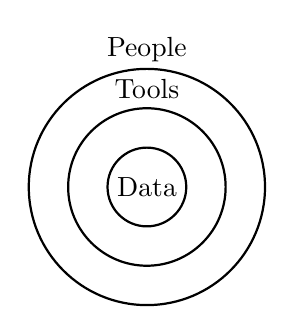
\begin{tikzpicture}
    \draw[thick] (0,0) circle (1.5cm);
    \draw[thick] (0,0) circle (1cm);
    \draw[thick] (0,0) circle (0.5cm);
    \node at (0,0) {Data};
    \node at (0,1.25) {Tools};
    \node at (0,1.75) {People};
    \end{tikzpicture}
    \end{frame}


\end{document}